\epigraph{\singlespacing \it ``It seems there is no problem in modern physics for which there are on record as many false starts, and as many theories which overlook some essential feature, as in the problem of the thermal conductivity of [electrically] non-conducting crystals.''}{R.~Peierls, 1960~\cite{Peierls1960}}


Conductive heat transport is the phenomenon of vibrational energy traversing a material when a temperature gradient is applied. As first described by Joseph Fourier in the early 19th century~\cite{Fourier1878}, the heat flux $\b J$ resulting from a stationary temperature gradient $\nabla T$ is directly proportional to this gradient. The proportionality constant is second-rank tensor denoted by $\kappa$ and called the \emph{thermal conductivity}. The defining equation,
\begin{align}
  \b J = - \kappa \nabla T~,
  \label{eq:Fourier}
\end{align}
is called \emph{Fourier's law}. The sign convention is such that the heat flows from ``hot to cold'' in compliance witht the second law of thermodynamics. The regime where Eq.\,\eqref{eq:Fourier} is valid is called the \emph{diffusive} regime, as it holds when the temperature gradient is small on microscopic scale, and the sample size is big enough so that boundary effects are negligible~\cite{Kapitza1941a,Antidormi2020}.

It is evident from Eq.\,\eqref{eq:Fourier} that the thermal conductivity $\kappa$ is an explicitly non-equilibrium quantity. As such, it can be related to equilibrium fluctuations by means of a \emph{fluctuation-dissipation theorem}~\cite{Einstein1905a,Nyquist1928,Callen1951,Kubo1957a}, resulting in the famous Green-Kubo formula~\cite{Green1952,Kubo1957b},
\begin{align}
  \kappa^{\alpha \beta} = \frac{V}{k_{\rm B} T^2} \int_{0}^{\infty} \d t ~
    \braket{J^\alpha (t) J^\beta(0)}_{\rm eq}~.
  \label{eq:GreenKubo}
\end{align}
This formula relates the temporal fluctuations of the macroscopic heat flux $\b J (t)$ as given by an equilibrium ensemble average of the autocorrelation function, $\braket{J^\alpha (t) J^\beta(0)}_{\rm eq}$, to the associated transport coefficient $\kappa$. It is however \emph{a priori} unclear how a microscopic description of the appearing quantities can be obtained. To tackle this question in full, we first show how the Kubo formula emerges in the framework of linear response theory. We then present how a microscopic description of heat in terms of a thermal energy density and an associated, locally conserved current follows, before reviewing the necessary steps to define an \emph{ab initio} heat flux~\cite{Carbogno2016}.

\section{Linear Response Theory}
The aim of linear response theory is to compute the expected value of a phase-space observable $B$ in presence of an external perturbation driving the system out of equilibrium. The ensemble is characterized by a \emph{distribution function} $f(\Gamma, t)$, where $\Gamma = \set{\b R, \b P}$ is a shorthand for a point in phase space. The expectation value of $B$ is given by
\begin{align}
  \braket{B (t)}_{f}
    = \int \d \Gamma ~ B (\Gamma) f(\Gamma, t)~,
  \label{eq:lr.B.1}
\end{align}
and we assume without loss of generality that its equilibrium value vanishes,
\begin{align}
\braket{B (t)}_{f^0}
= \int \d \Gamma ~ B (\Gamma) f^0(\Gamma) = 0~,
\label{eq:lr.B0}
\end{align}
where $f^0 (\Gamma)$ is the distribution function of the unperturbed system in thermal equilibrium. In order to calculate Eq.\,\eqref{eq:lr.B.1} in a non-equilibrium situation, we start by defining the Hamiltonian describing the dynamics of the system in the absence of external perturbations, $H^0$, which we take to be given by the many-body Hamiltonian
\begin{align}
  H^0 (\Gamma) 
    %= H^0(\set{\b R, \b P})
    = \sum_I \frac{\b P_I^2}{2 M_I} + V (\b R)~.
  \label{eq:lr.H0}
\end{align}
The canonical distribution function for the unperturbed system reads
\begin{align}
f^0 (\Gamma) 
= \frac{1}{\mathcal{Z}^0} {\rm e}^{- \beta H^0 (\Gamma)}~,
\label{eq:lr.f0}
\end{align}
where the partition sum $\mathcal{Z}_0$ normalizes the phase-space integral, \mbox{$\int \d \Gamma f^0 (\Gamma) = 1$}.
In the next step, we write the full Hamiltonian as
\begin{align}
  H (\Gamma, t)
   = H^0 (\Gamma) + \lambda H' (\Gamma, t)~,
  \label{eq:lr.H}
\end{align}
where the perturbation is given by some yet unspecified phase-space function $H' (\Gamma, t)$ with explicit time dependence, and $\lambda = 1$ is a bookkeeping parameter that we introduce to count the order in the perturbation.
We write the distribution function in presence of the perturbation as
\begin{align}
  f (\Gamma, t) = f^0(\Gamma) + \lambda \Delta f (\Gamma, t)~,
  \label{eq:lr.f}
\end{align}
where $\Delta f$ is the perturbation in the distribution generated by $H'$. Using that $f^0$ carries no explicit time dependence, the Liouville equation for $\Delta f$ reads
\begin{align}
  \lambda \frac{\d \Delta f}{\d t}
    &= \set{H, f} \nonumber \\
    &= \lambda \set{H^0, \Delta f} 
      + \lambda \set{H', f^0}
      + \mathcal{O}(\lambda^2)~,
  \label{eq:lr.df.1} \\
  \implies
    \frac{\d \Delta f}{\d t}
      &\approx \set{H^0 , \Delta f} + \set{H' (t), f^0}
  \label{eq:lr.df.2}
\end{align}
where $\set{\cdot , \cdot}$ denotes the Poisson bracket
%\footnote{
%  The Poisson bracket for a system of particles with $3N$ positions $q_i \equiv R_I^\alpha$ and conjugate momenta $p_i \equiv P_I^\alpha$ reads
%  $$
%  \set{A, B} = \sum_{i}
%  \frac{\partial A}{\partial q_i} \frac{\partial B}{\partial p_i}
%  - \frac{\partial A}{\partial p_i} \frac{\partial B}{\partial q_i}~.
%  $$
%  }, 
and in Eq.\,\eqref{eq:lr.df.2} we only keep the terms to linear order in the perturbation.
The solution to this differential equation is found to be\footnote{The solution is given in appendix \ref{app:lr.f}.}~\cite{Kubo1957a}
\begin{align}
  \Delta f (t) 
    = \int_{-\infty}^t {\rm e}^{-\im L^0 (t - t')} \set{H' (t'), f^0}~\d t'~,
  \label{eq:lr.df(t)}
\end{align}
where $\exp (\im L^0 t)$ propagates a phase-space point $\Gamma$ by a time $t$ according to the equations of motion following from $H^0$.
By splitting the interaction Hamiltonian $H'(t)$ into an operator part $A(\Gamma)$ and an explicitly time dependent force function $F(t)$,
\begin{align}
  H' (t)=AF(t)~,
\end{align}
this expression can be simplified in the canonical ensemble by using that \mbox{$\partial f^0 / \partial H^0 = -\beta f^0$}, which leads to
\begin{align*}
  \set{A, f^0}
%    &= \sum_i \frac{\partial A}{\partial q_i} \frac{\partial f^0}{\partial p_i}
%    - \frac{\partial A}{\partial p_i} \frac{\partial f^0}{\partial q_i} \\
%    &= \sum_i \frac{\partial A}{\partial q_i} \frac{\partial f^0}{\partial H^0} \frac{\partial H^0}{\partial p_i}
%    - \frac{\partial A}{\partial p_i} \frac{\partial f^0}{\partial H^0} \frac{\partial H^0}{\partial q_i} \\
%    &= -\beta f^0 \sum_i
%      \left( \frac{\partial A}{\partial p_i} \dot{q}_i +  \frac{\partial A}{\partial q_i} \dot{p}_i \right) \\
    &= -\beta f^0 \, \frac{\d A}{\d t}~.
\end{align*}
%where in the second step Hamilton's equations of motion have been used.

We are now in the position to formulate the expected response of a phase space observable $B$ to linear order in a perturbation described by the Hamiltonian $H'(t) = A F(t)$,~i.\,e.,~
\begin{align}
\braket{B (t)}_f
    &= \int \d \Gamma ~  B (\Gamma) \Delta f (\Gamma, t) \\
    &= - \beta \int_{-\infty}^t 
      \int \d \Gamma ~  
       B (\Gamma) \, {\rm e}^{-\im L^0 (\Gamma) (t - t')} \dot{A}(\Gamma)
       f^0(\Gamma) F(t') ~ \d t' \\
    &= - \beta \int_{-\infty}^t 
      \braket{B(t) \dot{A}(t')}_{f^0} F(t') ~ \d t'~,
  \label{eq:lr.dB}
\end{align}
where it was used that $a(t) = {\rm e}^{\im L^0 t} a(0) = a(0) {\rm e}^{-\im L^0 t}$~\cite[p.\,498]{Tuckerman}, and $\braket{\cdot}_{f^0}$ denotes a phase-space average with respect to the unperturbed canonical distribution function $f^0 (\Gamma)$. It is evident from this equation that the time propagation of the observables $\dot A$ and $B$ is generated by $L^0$ and therefore microcanonical with conserved energy. The phase-space average $\braket{\cdot}_{f^0}$ on the other hand corresponds to a canonical ensemble average with a defined inverse temperature $\beta$.

\subsection{Conserved densities and currents}
Macroscopic properties of matter are often \emph{extensive},~i.\,e.,~they scale with the system size, and can be described by a locally conserved \emph{density}. Taking the general property $A$ represented by the phase-space observable $A(\Gamma_t)$ evaluated at a time $t$ as an example, we define
\begin{align}
  A (\Gamma_t) = \int_V a (\b r, \Gamma_t) \, \d^3 r~,
  \label{eq:lr.A}
\end{align}
where $a(\b r, \Gamma_t)$ is the \emph{local density} associated with the observable $A$. The notation $\Gamma_t$ highlights that the quantity is implicitly time-dependent because the phase-space point $\Gamma$ evolves in time.
When no ambiguity arises, we can therefore just write $a (\b r, t)$.\footnote{
	Notation for phase-space functions $f (\Gamma)$:
	\begin{align*}
	f(t) &\equiv f(\Gamma (t)) \\
	\frac{\partial f}{\partial t} &= \frac{\d f (\Gamma (t))}{\d t} \equiv \dot{f}(t)
	\end{align*}
}
The locally conserved density fulfills a continuity equation
\begin{align}
  \partial_t \, a(\b r, t) = - \b \nabla \cdot \b j_a (\b r, t)~,
  \label{eq:lr.continuity.1}
\end{align}
where $\b j_a (\b r, t)$ is the associated current. From the local current, the macroscopic flux is obtained by spatially averaging over the system volume,
\begin{align}
  \b J (t)
    = \frac{1}{V} \int_V \d^3 r ~ \b j (\b r, t)~,
  \label{eq:lr.J(t)}
\end{align}
where the subscript $a$ was dropped for notational clarity.
Likewise we formulate a local version of the perturbing Hamiltonian \mbox{$H' = A (\Gamma) F(t)$} in the form
\begin{align}
	H' (\Gamma, t) = \int \d^3 r ~ a (\b r, \Gamma) v(\b r, t)~,
	\label{eq:lr.H'}
\end{align}
where $a(\b r, \Gamma)$ represents the density of interest as introduced above, and $v(\b r, t)$ is the local driving force coupling to the system via the density $a (\b r, \Gamma)$.

The local version of linear-response formula given in Eq.\,\eqref{eq:lr.dB} with \mbox{$\Delta B = B \equiv \b J$} reads:\footnote{Remember 
	$\braket{B} \equiv \braket{\b J} = 0$~.}
\begin{align}
j^\alpha (\b r , t) 
	& \equiv \braket{j^\alpha (\b r)}_{\Delta f (t)} \\
	&= - \beta \int_{-\infty}^{t} \d t' \int_V \d^3 r' ~ \braket{
			j^\alpha (\b r, \Gamma_t) \dot{a} (\b r', \Gamma_{t'})
		}_0 v (\b r', t')~.
	\label{eq:lr.ja.1}
\end{align}
The time derivative of the density can be eliminated by using the continuity equation~\eqref{eq:lr.continuity.1}, $\dot a = \partial'_\beta j^\beta$ where $\partial'_\beta = \partial/\partial r^{\prime \beta}$, and integrating by parts, so that
\begin{align}
j^\alpha (\b r , t) 
&= - \beta \int_{-\infty}^{t} \d t' \int_V \d^3 r' ~ \braket{
	j^\alpha (\b r, \Gamma_t) j^\beta (\b r', \Gamma_{t'})
}_0 \partial'_\beta v (\b r', t')~.
\label{eq:lr.ja.2}
\end{align}
If we now assume the external driving force $v (\b r, t)$ to be constant in time and homogeneously varying in space such that
\begin{align}
	\partial_\beta v (\b r, t) \equiv v_\beta~,
	\label{eq:lr.force}
\end{align}
and spatially average over Eq.\,\eqref{eq:lr.ja.2} with $\frac{1}{V} \int_V \d^3 r$, we arrive at
\begin{align}
	J^\alpha 
		&= -\beta V \int_{0}^{\infty} 
		\d t
		\braket{
		J^\alpha (\Gamma_t) J^\beta (\Gamma_{0})
	}_0 
	v_\beta~,
	\label{eq:lr.J}
\end{align}
where the stationarity in time was used to shift the lower bound of the integral to $t=0$.
This resembles the well-known macroscopic transport equation
\begin{align}
	J^\alpha =  L^{\alpha \beta} F_\beta~,
		\label{eq:lr.LF}
\end{align}
with
\begin{align}
	L^{\alpha \beta}
		= \frac{V}{k_{\rm B}} \int_{0}^{\infty} 
		\d t \braket{J^\alpha (\Gamma_t) J^\beta (\Gamma_{0})}_0 ~,
	\label{eq:lr.L}
\end{align}
and
\begin{align}
	F_\beta
		= - \frac{v_\beta}{T}~.
	\label{eq:lr.F}
\end{align}
Here, $J^\alpha$ is the macroscopic generalized current associated with the extensive property $A$, $F_\beta$ is the thermodynamic force, and $L^{\alpha \beta}$ is the associated conductance tensor~\cite{Onsager1931a,Baroni2020a}.

\subsection{Thermal Conductivity}
\label{sec:Thermal.Conductivity}
After this general exposition, let us now look at the example of the total energy of the system and its associated energy density,
\begin{align}
	E = \int_V \d^3 r ~ e(\b r)~.
	\label{eq:lr.E}
\end{align}
We are interested in the occuring flux in the presence of an inhomogeneous temperature, $T(\b r) = T + \Delta T(\b r)$, which couples linearly to the energy density  $e (\b r)$, so that\footnote{$E$ and $H(\Gamma)$ are related by $E = \braket{H}$. The same holds for the occurring densities $e(\b r)$ and $e (\b r, \Gamma)$.}
\begin{align}
	H (\Gamma) = \frac{1}{T} \int \d^3 r ~ T (\b r) e(\b r, \Gamma) 
		\equiv H^0 (\Gamma) + H' (\Gamma)~,
\end{align}
with
\begin{align}
	H' (\Gamma) = \frac{1}{T} \int \d^3 r ~ \Delta T (\b r) e(\b r, \Gamma)~.
	\label{eq:lr.Hp.temp}
\end{align}
With the previous assumption that $\Delta T(\b r)$ varies linearly in space, we find the thermodynamic force to be given by
\begin{align}
	v_\beta = \frac{1}{T} \partial_\beta T (\b r) 
		\stackrel{\eqref{eq:lr.F}}{\implies}
	F_\beta = - \frac{1}{T^2} (\b \nabla T)_\beta ~.
	\label{eq:lr.F.temp}
\end{align}
Using the general transport equation $\b J = L \b F$ with the conductance given by Eq.\,\eqref{eq:lr.L} and $F$ as defined above, we obtain
\begin{align}
	J^\alpha 
		&= - \kappa^{\alpha \beta} (\b \nabla T)_\beta~,
	\label{eq:lr.J.2}
\end{align}
where $\kappa^{\alpha \beta}$ denotes the \emph{thermal conductivity tensor} defined as
\begin{align}
	\kappa^{\alpha \beta}
		&=
		\frac{V}{k_{\rm B} T^2} \int_{0}^{\infty} 
		\d t \braket{J^\alpha (\Gamma_t) J^\beta (\Gamma_{0})}_0 ~,
	\label{eq:GreenKubo}
\end{align}
that is, the Green-Kubo formula for the thermal conductivity $\kappa$.

\section{Heat Flux Definition}
In order to evaluate the thermal conductivity by means of the Green-Kubo formula, Eq.\,\eqref{eq:GreenKubo}, the  heat flux observable $\b J (\Gamma)$ needs to be defined. We do so by starting from the continuity equation again,
\begin{align}
	\dot{e} (\b r) = - \b \nabla \cdot \b j (\b r)
	\label{eq:hf.cont}
\end{align}
and perform a Fourier transform in space defined by the pair of equations
\begin{align}
	e(\b r) 
		&= \int \d^3 q ~ e(\b q) \, {\rm e}^{\im \b q \cdot \b r} ~,
		\label{eq:hf.ft.r} \\
	\Leftrightarrow
	e(\b q) 
		&= \frac{1}{V} \int \d^3 r ~ e(\b r) \, {\rm e}^{-\im \b q \cdot \b r} ~,
	\label{eq:hf.ft.2}
\end{align}
so that the continuity equation can be rewritten for the Fourier components as
\begin{align}
	\dot{e} (\b q)
		= - \im \b q \cdot \b j (\b q)~.
	\label{eq:hf.ft.cont.q}
\end{align}
We split the total current into a longitudinal, heat-carrying component $\b j_{\parallel}$ and a transverse current $\b j_{\perp}$,
\begin{align}
	\b j = \frac{\b q}{q} j_{\parallel} + \b j_{\perp} \quad\text{where}\quad \b q \cdot \b j_{\perp} = 0~,
\end{align}
so that
\begin{align}
	\b j_{\parallel} (\b q)
		= \im \frac{\b q}{q^2} \dot{e} (\b q)~.
  \label{eq:hf.j.parallel}
\end{align}
As before, we obtain the macroscopic heat flux as a spatial average of the (longitudinal) current,
\begin{align}
	\b J (t) = \frac{1}{V} \int \d^3 r ~ \b j_{\parallel} (\b r) = \b j_{\parallel} (\b q \to 0)~,
	\label{eq:hf.J.1}
\end{align}
where it was used that, by definition of the Fourier transform, the integral over the system volume equals the long wavelength limit of the current in reciprocal space. The long wavelength limit for the time derivative of the local energy density can be obtained by Taylor expanding in $\b q$
\begin{align}
	\dot{e} (\b q) 
		= \lim_{\b q \to 0} \int \d^3 r \left(\cancel{1} - \im \b q \cdot \b r + (\b q \cdot \b r)^2 + \cdots \right) \dot{e} (\b r)~,
	\label{eq:hf.e.lw}
\end{align}
where the first term in the expansion is excluded since the total energy $E$ is conserved in time.\footnote{Use Leibniz rule:
\begin{align*}
	\int \d^3 r \, \dot{e} (\b r) = \frac{\d}{\d t} \int \d^3 r \, e (\b r) = \frac{\d}{\d t} E = 0
\end{align*}
}
After multiplying $\dot e$ with $\im \b q / q^2$ according to Eq.\,\eqref{eq:hf.j.parallel} and taking the $\b q \to 0$ limit, we obtain
\begin{align}
	\b J (t) 
		= \frac{1}{V} \int \d^3 r ~ \b r \, \dot{e} (\b r, t)
		= \frac{1}{V} \frac{\d}{\d t} \int \d^3 r ~ \b r \, e (\b r, t)
	~,
	\label{eq:hf.J}
\end{align}
i.\,e.,~the heat flux is given as the first moment of the time derivative of the local energy density. Alternatively, one can view the heat flux as the time derivative of the energy barycenter by moving the time derivative outside the integral.

In force-field approaches, it is common to adopt the latter approach and split the energy density into atomic contributions as
\begin{align}
	e (\b r, t ) = \sum_I E_I (t) \delta (\b r - \b R_I)~.
	\label{eq:hf.e.atomic}
\end{align}
The heat flux is then given by~\cite{Helfand1960}
\begin{align}
	\b J (t) 
		= \frac{1}{V} \frac{\d}{\d t} \sum_I E_I(t) \b R_I(t)
		% = \frac{1}{V} \sum_I \dot{E}_I (t) \b R_I (t) + E_I (t) \dot{\b R}_I (t)~,
		= {\bf J}^{\rm pot} (t) + {\bf J}^{\rm kin} (t)~,
	\label{eq:hf.J.atomic}
\end{align}
with a \emph{potential} or \emph{virial} current
\begin{align}
	{\bf J}^{\rm pot} (t)
		= \frac{1}{V} \sum_I \dot{E}_I (t) \b R_I (t)~,
	\label{eq:J_pot}
\end{align}
and a \emph{kinetic} or \emph{convective} current
\begin{align}
	{\bf J}^{\rm kin} (t)
		= \frac{1}{V} \sum_I E_I (t) \dot{\b R}_I (t)~.
	\label{eq:J_kin}
\end{align}
In non-convective solids, the kinetic contribution is typically neglected, as it was shown several times in the literature that its contribution to thermal conductivity is orders of magnitude lower compared to the virial flux~\cite{Vogelsang1987,Kinaci2012}. However, the kinetic flux becomes increasingly important and even dominant in liquids and gases with substantial convection~\cite{Cheng2020}.

\subsection{Gauge invariance of heat flux definitions}
As seen above, the local current is only defined up to a non-heat carrying contribution $\b j_{\perp}$. Likewise, the energy density is only defined up to terms that keep the total energy integral unchanged. The choice of a local energy partitioning as,~e.\,g.,~given by Eq.\,\eqref{eq:hf.e.atomic} is therefore not unique, and different partitioning schemes will lead to differing heat fluxes. However, the thermal conductivity obtained by these heat fluxes will be the same in the long time limit. In particular, Ercole \emph{et al.} have shown in Ref.\,\cite{Ercole2016} that two heat fluxes differing by the time derivative of a \emph{bounded} vector field,
\begin{align}
  \tilde{\b J} (t) = \b J (t) + \frac{\d}{\d t} \b P (t)~,
\end{align}
can differ in time, and in general also their autocorrelation functions will differ. The thermal conductivity obtained from both fluxes will however be the same, which can be viewed as a \emph{gauge invariance principle} for the heat flux. This property can be used to discard terms from the flux that do not contribute to the thermal conductivity and thereby reduce noise~\cite{Marcolongo2020}. 
%We will show practical implications of this ``gauge invariance principle'' later in the results part.

\newthought{As an example of immediate practical importance}, we rewrite the heat flux expression presented in Eq.\,\eqref{eq:hf.J.atomic} as
\begin{align}
	\b J (t) 
%		&= \frac{1}{V} \sum_I \left[ \b R_I^0 \fD{\dot{E}}_I + \b U_I \dot{E}_I + \dot{\b U}_I E_I\right] \\
	&= \frac{1}{V} \sum_I \b R_I^0 \fD{\dot{E}}_I + { \frac{1}{V} \frac{\d}{\d t} \sum_I \b U_I E_I}~,
	\label{eq:J_gauge_1}
\end{align}
where the instantaneous positions ${\bf R} (t)$ are split into a fixed reference ${\bf R}^0$ and a displacement field ${\bf U} (t)$~\cite{Isaeva2019}. When all the atomic displacements $\set{{\bf U}_I}$ are bounded,~i.\,e.,~in the absence of convective terms, the second term in Eq.\,\eqref{eq:J_gauge_1} fulfills the condition of being the time derivative of a bounded vector field and therefore does not contribute to the thermal conductivity by the gauge invariance principle. Using the definition of the kinetic flux in Eq.\,\eqref{eq:J_kin}, the second, non-contributing term can be written as
\begin{align}
	\frac{1}{V} \frac{\d}{\d t} \sum_I \b U_I E_I
		= {\bf J}^{\rm kin} + {\bf J}^{\rm res}
	\label{eq:J_gauge_2}
\end{align}
with a residual flux %${\bf J}^{\rm res} = \frac{1}{V} \sum_I \b U_I \dot E_I$
\begin{align}
	{\bf J}^{\rm res} (t)
		= \frac{1}{V} \sum_I \b U_I \dot E_I~.
	\label{eq:J_gauge_3}
\end{align}
This makes clear that, in the absence of convection, the contribution of ${\bf J}^{\rm kin}$ to thermal conductivity does not vanish alone, but only the \emph{joint} contribution of ${\bf J}^{\rm kin}$ and ${\bf J}^{\rm res}$. By the reverse argument, one can argue that whenever the contribution of ${\bf J}^{\rm kin}$ to thermal conductivity can be neglected in a solid, the contribution of ${\bf J}^{\rm res}$ must vanish as well. In consequence, the heat flux in non-diffusing solids is given by
\begin{align}
	\b J (t) 
		&= \frac{1}{V} \sum_I \b R_I^0 \fD{\dot{E}}_I
		\approx {\bf J}^{\rm pot} (t).
	\label{eq:J_tot_solid}
\end{align}
A final remark concerning this equation is in order: One might argue that the expression in Eq.\,\eqref{eq:J_tot_solid} is a total time derivative of ${\bf P} = \frac{1}{V}  \sum_I {\bf R}_I^0 \fD E_I$, and therefore vanishes by the aforementioned gauge invariance principle. However, this is not the case in an infinite solid, since the atomic configuration $\set{{\bf R}_I}$ is not bounded. The sum over atomic positions is therefore not well defined in the first place and remains to be understood as a symbolic representation of an actual energy partitioning scheme that needs to be cast in a boundary-insensitive form for any practical application of Eq.\,\eqref{eq:J_tot_solid}.\footnote{The author thanks Stefano Baroni for an insightful discussion clarifying this point.}

\section{Ab initio Heat Flux}
The above formulas are readily applied when empirical force fields are used to describe the atomic interactions, as an atomic partitioning of the total energy is trivial in that case, although care must be taken in deriving the correct formulae nevertheless~\cite{Fan2015,Boone2019}. An \emph{ab initio} derivation of heat flux on the other hand was a long-standing problem because it was not clear how an expression like Eq.\,\eqref{eq:J_tot_solid} can be obtained when no atomic partitioning is available. This problem was solved when Marcologno \emph{et al.} and Carbogno \emph{et al.} independently arrived at well-defined heat flux expressions in \emph{ab initio} frameworks~\cite{Marcolongo2016,Carbogno2016}. We adopt the latter approach in the following, but present a derivation that slightly differs from Ref.\,\cite{Carbogno2016},~i.\,e.,~by starting from Eq.\,\eqref{eq:hf.J} instead of Eq.\,\eqref{eq:hf.J.atomic}, and using the phase-space formalism developed in this chapter.

% \paragraph{Derivation of ab initio Heat Flux}
To evaluate Eq.\,\eqref{eq:hf.J},\footnote{Recall Eq.\,\eqref{eq:hf.J}:$$\b J (t) 
	= \frac{1}{V} \int \d^3 r ~ \b r \, \dot{e} (\b r, t)~.$$} we need a definition of the time derivative of the energy density. We do so by first going back to the many-body Hamiltonian for a configuration $\Gamma = (\b R, \b P)$ given by
\begin{align}
	H (\Gamma) = \sum_I \frac{\b P_I^2}{2 M_I} + V(\b R) 
		~\equiv~ \int \d^3 r ~ e (\b r, \Gamma)~,
  \label{eq:hf.ai.H}
\end{align}
where $e (\b r, \Gamma)$ is an appropriately chosen energy density yielding the total energy of the given system. Accordingly, the time derivative of the entire expression reads
\begin{align}
	\dot{H} (\Gamma)
		= \sum_I \b F_I \cdot \dot{\b R}_I 
		+ \sum_I \frac{\partial V(\b R)}{\partial \b R_I} \cdot \dot{\b R}_I
			\label{eq:hf.ai.Hdot}
		\stackrel{!}{\equiv}
			\int \d^3 r ~ \dot{e} (\b r , \Gamma)~.
\end{align}
We note in passing that the energy is supposed to be conserved so that the time derivate of the Hamiltonian vanishes, and therefore $\dot{e} (\b r, \Gamma)$ needs to integrate to zero.
As explained in Sec.\,\ref{sec:HellmannFeynman}, the force derived from the BO potential-energy surface $V ({\bf R})$ appearing in Eq.\,\eqref{eq:hf.ai.Hdot} has a nuclear and an electronic contribution given by the two terms in Eq.\,\eqref{eq:hellmannfeynman.force}, so that
\begin{align}
	\b F_I
		&%= - \frac{\partial V (\b R)}{\partial \b R_I}  
			= \int \d^3 r ~ \b f_I^{\rm el} (\b r) + \sum_{J \neq I} \b F_{IJ}^{\rm Nuc}~, \quad\text{with}
		\label{eq:hf.ai.F}\\
	\b f_I^{\rm el} (\b r)
		&= - n(\b r) Z_I \frac{\b R_I - \b r}{\lvert \b R_I - \b r \rvert^3}~,
		\label{eq:hf.ai.Fel}
		\quad\text{and} \\
	\b F_{IJ}^{\rm Nuc}
		&= Z_I Z_J \frac{\b R_I - \b R_J}{\lvert \b R_I - \b R_J \rvert^3}~.
		\label{eq:hf.ai.Fnuc}
\end{align}
Therefore, Eq.\,\eqref{eq:hf.ai.Hdot} can be written as the sum of three terms that sum to zero as required,
\begin{align}
	\dot{H} (\Gamma)
		&= \underset{I)}{\underbrace{\sum_I \b F_I \cdot \dot{\b R}_I}} ~ 
			 \underset{II)}{\underbrace{-\sum_{I} \int \d^3 r ~ \b f_I^{\rm el} (\b r) \cdot \dot{\b R}_I}} ~
			 \underset{III)}{\underbrace{-\sum_{\substack{I, J \\ J \neq I}} \b F^{\rm Nuc}_{IJ} \cdot \dot{\b R}_I}}~.
\end{align}
We use these terms to define three contributions to the local density $\dot{e} (\b r)$ as
\begin{subequations}
\begin{align}
	\text{I):}&&
		\dot{e}^{\rm kin} (\b r) &= \sum_I \b F_I \cdot \dot{\b R}_I \, \delta (\b R_I - \b r)~, \\
	\text{II):}&&
		\dot{e}^{\rm el} (\b r)  &= -\sum_{I} \b f_I^{\rm el} (\b r) \cdot \dot{\b R}_I~, \\
	\text{III):}&&
		\dot{e}^{\rm Nuc} (\b r) &= -\sum_{\substack{I, J \\ J \neq I}} \b F^{\rm Nuc}_{IJ} \cdot \dot{\b R}_I \, \delta (\b R_J - \b r)~.
\end{align}
\label{eq:hf.ai.densities}
\end{subequations}
Pictorially, the kinetic contribution $\dot{e}^{\rm kin} (\b r)$ is assigned to atom $I$ in the sum, the electronic contribution $\dot{e}^{\rm el} (\b r)$ is assigned to the local electron density at $\b r$ and is therefore a local quantity per definition, and the nuclear contribution $\dot{e}^{\rm Nuc} (\b r)$ is assigned to atom $J$ in analogy to the electronic case. It is easily verified that the sum of these contributions integrate to zero. Their first moment however gives a non-vanishing heat flux by Eq.\,\eqref{eq:hf.J},~i.\,e.,
\begin{align}
	\b J (\Gamma)
		% &= \frac{1}{V} \int \d^3 r ~ \b r \, \dot{e} (\b r, \Gamma) \\
		&= \frac{1}{V} \int \d^3 r ~ \b r \left( \dot{e}^{\rm kin} (\b r) + \dot{e}^{\rm el} (\b r) + \dot{e}^{\rm Nuc} (\b r)  \right) \\
		&= \frac{1}{V} \sum_I
			\left( 
				\b R_I \b F_I \cdot \dot{\b R}_I
				- \int \d^3 r ~ \b r \, \b f_I^{\rm el} (\b r) \cdot \dot{\b R}_I
				- \sum_{J \neq I} \b R_J \b F^{\rm Nuc}_{IJ} \cdot \dot{\b R}_I
			\right)~.
\end{align}
By using Eq.\,\eqref{eq:hf.ai.F} in the first summand of the above equation, Eq.\,\eqref{eq:hf.ai.Fel} for the second, and Eq.\,\eqref{eq:hf.ai.Fnuc} for the third, we arrive at
\begin{align}
	J^\alpha (\Gamma) \nonumber
		=  \sum_{I, \alpha} \frac{Z_I}{V}
			&\left\{ 
				\sum_{J \neq I} Z_J \frac{(R_I^\alpha - R_J^\alpha) (R_I^\beta - R_J^\beta)}{\lvert \b R_I - \b R_J \rvert^3} \right. \nonumber \\
				&~\left.- \int \d^3 r ~ n(\b r) \frac{(R_I^\alpha - r^\alpha) (R_I^\beta - r^\beta)}{\lvert \b R_I - \b r \vert^3}
			\right\}
			\dot{R}^\beta_I~,
	\label{eq:hf.ai.J}
\end{align}
where the Cartesian indices of the expressions have been restored.
As shown in Ref.\,\cite{Carbogno2016}, this expression can be written in terms of atomic contributions to the stress tensor $\sigma$ defined by
\begin{align}
  \sigma^{\alpha \beta} 
    = - \frac{\partial V ({\bf R})}{\partial \varepsilon_{\alpha \beta}}
    = \sum_I \sigma_I^{\alpha \beta}~,
  \label{eq:hf.sigma}
\end{align}
with
\begin{align}
  \sigma_I^{\alpha \beta}
    = \frac{Z_I}{V}
        \left\{ 
        \sum_{J \neq I} Z_J \frac{(R_I^\alpha - R_J^\alpha) (R_I^\beta - R_J^\beta)}{\lvert \b R_I - \b R_J \rvert^3}
        - \int \d^3 r ~ n(\b r) \frac{(R_I^\alpha - r^\alpha) (R_I^\beta - r^\beta)}{\lvert \b R_I - \b r \vert^3}
        \right\}~.
  \label{eq:hf.sigma_I}
\end{align}
This can be rationalized by using the same steps that led to the Hellmann-Feynman expression for the position derivative in Eq.\,\eqref{eq:hellmannfeynman.force}, and noting that
\begin{align}
  \frac{\partial f (\b r_1 - \b r_2)}{\partial \varepsilon_{\alpha \beta}}
    = \frac{\partial f (\b r_1 - \b r_2)}{\partial r_1^\alpha} (r_1^\beta - r_2 ^\beta)~,
  \label{eq:strain.derivative}
\end{align}
as discussed in detail in Ref.\,\cite{Knuth2015}.
The atomic stress contributions $\sigma_I$ are functionals of the electron density and atomic configuration and as such straightforward to compute in \emph{ab initio} frameworks, for example in the all-electron, numeric atomic orbital electronic structure code \emph{FHI-aims}~\cite{FHI-aims,Knuth2015}. The final result for the \emph{ab initio} heat flux used in this work is therefore
\begin{align}
	{\bf J}^{\rm ai} (t) = \sum_I \sigma_I (t) \dot{\bf R}_I~,
	\label{eq:J_ai}
\end{align}
where $\sigma_I (t)$ is Eq.\,\eqref{eq:hf.sigma_I} evaluated for the configuration ${\bf R} (t)$.

\newthought{To conclude, we like to point out} that by using the time derivative of the energy density, we neglect convective contributions to the flux from the very beginning. The present \emph{ab initio} heat flux is therefore valid for solids with vanishing or negligible mass diffusion.

\CITE{[1] O. H. Nielsen and R. M. Martin, Phys. Rev. B 32, 3780 (1985).?}

\section{Heat Flux in the Harmonic Approximation}
We now discuss heat flux in the harmonic approximation. This work was pioneered by Debye and Peierls~\cite{Debye1914,Peierls1929}, with a formal derivation first presented by Hardy~\cite{Hardy1963}. 

\newthought{We start from the gauge-invariant heat flux expression} for solids as defined in Eq.\,\eqref{eq:J_tot_solid},~i.\,e.,
\begin{align}
	\b J (t) 
		= \frac{1}{V} \sum_I \b R_I^0 \fD{\dot{E}}_I~.
		\label{eq:J_ha_0}
\end{align}
The atomic energy contribution $E_I$ expressed in mass-scaled displacements $\set{\b u_I}$ and momenta $\set{\b p_I}$ reads
\begin{align}
	E_I = \halb p_I^2 + \halb \sum_J D_{I \alpha , J \beta} \, u_I^\alpha u_J^\beta~,
\end{align}
with the dynamical matrix $D_{IJ}$, so that\marginnote{The harmonic forces are
	\begin{align*}
	\dot{p}_{I\alpha}
	= - \frac{\partial E}{\partial u_I^\alpha} 
	= - \sum_J D_{I \alpha , J \beta} \, u_J^\beta~,
	\end{align*}
and in mass-weighted coordinates
	$$\dot{u}_I^\alpha = p_I^\alpha~.$$
}
\begin{align}
	\dot E_I 
		&= \sum_J \dot{p}_{I\alpha} p_I^\alpha 
		+ \halb \sum_J D_{I \alpha , J \beta} \, 
			\left( p_I^\alpha u_J^\beta + u_I^\alpha p_J^\beta\right) \nonumber \\ 
		&= -\halb \sum_J D_{I \alpha , J \beta} \, 
		\left( p_I^\alpha u_J^\beta - u_I^\alpha p_J^\beta\right) ~.
		\label{eq:dotE_I}
\end{align}
Using this expression for the time derivative of the atom-resolved harmonic energy  in Eq.\,\eqref{eq:J_ha_0} leads to a heat flux of the form
\begin{align}
    \b J^{\rm ha-r} (t) = - \frac{1}{2V} \sum_{IJ} (\b R_I^0 - \b R_J^0) D_{I \alpha, J \beta} \, p_I^\alpha (t) u_J^\beta (t)~,
   \label{eq:J_ha_r}
\end{align}
which is boundary-insensitive as required since only differences of positions enter.
By expressing the displacements $\set {\b u_I}$ and velocities $\set{\b p_I}$ in terms of the complex mode amplitudes $a_s (t)$ introduced in Eq.\,\eqref{eq:u_s.amplitudes.periodic} in Sec.\,\ref{sec:dynmat.periodic},
\begin{align}
    \b u_I (t) 
	    &= ~\sum_s \frac{1}{\sqrt{2 \omega_s}} \b e^\ast_{s I} \left[ \D a_{-s} (t) + \fD a_s (t)\right]~,\quad\text{and} \\
	  \b p_I (t) 
		  &= \sum_s ~\im \sqrt{\frac{\omega_s}{2}} ~ {\b e}_{s I} \left[ \D a_{-s} (t) - \fD a_s (t) \right]~,
\end{align}
the harmonic heat flux reads
\begin{align}
    \b J^{\rm ha-q} (t) 
	    %&= \halb \sum_{ss'} \b v_{ss'} \omega_{s} \D u_s (t) p_{s'} (t) \\
	    &= \frac{1}{2V} \sum_{ss'} \b v_{ss'} \omega_{s} \left( \D a_{-s} + \fD a_{s}  \right) \left( \D a_{s'} - \fD a_{-s'}  \right)~,
	  \label{eq:J.ha}
\end{align}
with the generalized group velocity
\marginnote{With the shorthand notation $s=(b, \b q)$ and $I = (i, \b L)$, we find that the diagonal term $\b v_s = \b v_{ss'}$ is indeed the group velocity:
	\begin{align*}
		\b v_{s} 
			&= \frac{\partial \omega_s}{\partial \b q}  = \frac{1}{2 \omega_s} \frac{\partial \omega_s^2}{\partial \b q} \\
			&= \frac{1}{2 \omega_s} \sum_{ij} e^\ast_{s, i \alpha} \frac{\partial D_{i \alpha, j \beta} (\b q)}{\partial \b q} e_{s, j \beta} \\
			&= \frac{1}{2 \omega_s} \sum_{I, J} \im \left( \b R^0_{I} - \b R^0_{J} \right)
			D_{I \alpha, J \beta}	e^\ast_{s, I \alpha} e_{s, J \beta}~.
	\end{align*}}
\begin{align}
	\b v_{ss'}
		&= \frac{1}{2 \sqrt{\omega_s \omega_{s'}}} \sum_{IJ} \im (\b R^0_I - \b R^0_J) D_{I \alpha, J \beta} e^\ast_{s, I \alpha} \fD e_{s', J \beta}~.
\end{align}
Using that $\b v (- \b q) = - \b v (\b q)$, %and defining the mode occupation \mbox{$n_s (t) \equiv \D a_s (t) \fD a_s (t)$}, 
the diagonal contribution ($s=s'$) to the flux reads
\begin{align}
	\b J^{\rm ha-q-diag} (t) 
%		= \halb \sum_{s} \fD{\b v}_{s} \fD \omega_{s} \D p_s (t) u_{s} (t)
		= \frac{1}{V} \sum_{s} \fD {\b v}_{s} \omega_{s} ~ \D a_s (t) \fD a_s (t)
		\equiv \frac{1}{V} \sum_{s} E_s (t)  {\bf v}_{s}~,
	\label{eq:J.ha.diag}
\end{align}
where the mode energy $E_s = \omega_s \D a_s \fD a_s$ was used.
This result is the familiar phonon heat flux operator first derived by Hardy~\cite{Hardy1963}.\footnote{Via the identification $E_s = \omega_s n_s$ (when setting $\hbar = 1$)~.}

\newthought{With the harmonic heat flux at hand}, it is straightforward to show that the thermal conductivity of a purely harmonic system is infinite. At the same time, useful approximations to compute the thermal conductivity from a perturbation theory perspective can be found. We demonstrate the reasoning for the case of the diagonal contribution to the heat flux $\b J^{\rm ha-q-diag}$ given by Eq.\,\eqref{eq:J.ha.diag}, which we simply denote by $\bf J$ in the following. The additional terms stemming from the offdiagonal contribution to the heatflux have been worked out in Ref.\,\cite{Isaeva2019}.

As discussed in detail in Sec.\,\ref{sec:Thermal.Conductivity}, the thermal conductivity is given by the Kubo formula
\begin{align}
	\kappa
		&=
		\frac{V}{k_{\rm B} T^2} \int_{0}^{\infty} 
		\d t \braket{J (t) J} ~,
\end{align}
where we have omitted the Cartesian components for clarity.
The contribution from the diagonal harmonic heatflux therefore reads
%\footnote{We simply denote $J \equiv J^{\rm ha-q-diag}$ in the following.}
\begin{align}
    \braket{J(t) J} = \frac{1}{V^2} \sum_{ss'} \omega_s \omega_{s'} v_{\fP s} v_{s'}
	    \braket{\D a_s (t) \fD{a}_s (t) \D a_{s'} \fD a_{s'}}~.
	   \label{eq:ha.kappa.J.corr}
\end{align}
The expectation value $\braket{\cdot}$ can be viewed as a functional integral with the distribution function $f = {\rm e}^{-\beta \sum_s \omega_s \D a_{s} \fD a_{s}}$ and can therefore be evaluated by means of a Wick theorem.\footnote{In the context of complex field integration, the Wick theorem reads~\cite{Negele2018} $$\braket{ABCD} = \braket{AB}\braket{CD} + \braket{AC}\braket{BD} + \braket{AD}\braket{BC}.$$}
Keeping only the non-vanishing pairings, we have
\begin{align}
	\braket{\D a_s (t) \fD{a}_s (t) \D a_{s'} \fD a_{s'}}
		= \braket{n_s} \braket{n_{s'}} + \fD g_s (t) g^\ast_{s} (t) \delta_{ss'}~,
	\label{eq:ha.kappa.wick}
\end{align}
where $\braket{n_s} = \frac{k_{\rm B} T}{\omega_s}$
%\begin{align}
%	\braket{n_s} = \frac{k_{\rm B} T}{\omega_s}
%\end{align}
is the classical mode occupation, and the one-particle Green's function $g_s (t)$ is defined by
\begin{align}
	g_s (t) \delta_{ss'}
		\equiv \braket{\D{a}_{\fP s} (t) \fD{a}_{s'}} 
		= {\rm e}^{\im \omega_s t} \braket{n_s} \delta_{ss'}~,
\end{align}
where the time evolution of the complex amplitudes $a^{\dagger} (t) = {\rm e}^{\im \omega_s t} \D a_s$ was used.
It is apparent that the correlation function defined in Eq.\,\eqref{eq:ha.kappa.wick} is not time-dependent, and the heatflux autocorrelation function defined in Eq.\,\eqref{eq:ha.kappa.J.corr} is given by
\begin{align}
	\braket{J (t) J} = \cancel{\braket{J}^2} + \sum_s \braket{J_s^2}~.
	\label{eq:ha.kappa.JJ}
\end{align}
In thermodynamic equilibrium, the expectation value of the heatflux, $\braket{J}$, vanishes, the mode variance $J_s^2$ however does not vanish. The harmonic heatflux autocorrelation function therefore integrates to infinity and the thermal conductivity $\kappa$ diverges.

\newthought{A finite thermal conductivity} is obtained when the phonons are allowed to interact, for example by introducing impurities, electron-phonon interactions, or self interactions via anharmonic contributions to the potential-energy surface. If the perturbation is weak, it can be expressed by modified Green's functions
\begin{align}
	g_s (t) = {\rm e}^{\im \left( \omega_s + \Sigma_s \right) t} \braket{n_s}~,
	\label{eq:ha.kappa.g.self}
\end{align}
where $\Sigma_s$ is the phonon self energy. Assuming the self energy to be purely imaginary, $\Sigma_s = \im \Gamma_s$, we have
\begin{align}
	\fD g_s (t) g^\ast_{s} (t) = {\rm e}^{- 2 \Gamma_s t} \braket{n_s}^2
	\equiv {\rm e}^{-t / \tau_s} \braket{n_s}^2~,
	\label{eq:ha.kappa.gg.Sigma}
\end{align}
where he have defined the lifetime $\tau_s = 1 / 2 \Gamma_s$. The heatflux autocorrelation function now reads
\begin{align}
	\braket{J (t) J} = \sum_s \braket{J_s^2} {\rm e}^{-t / \tau_s}~,
	\label{eq:ha.kappa.JJ.pert}
\end{align}
and the thermal conductivity integrates to a finite value given by\marginnote{Using $$J_s = \omega_s v_s n_s$$ and $$\braket{n_s} = \frac{k_{\rm B} T}{\omega_s}~.$$}
\begin{align}
	\kappa^{\alpha \beta} = V k_{\rm B} \sum_{s} v^\alpha_s v^{\beta \vphantom{\dagger}}_s \fD \tau_s~.
	\label{eq:ha.kappa.bte}
\end{align}
The same expression can be found from a Boltzmann transport approach using the \emph{single-mode relaxation-time approximation}~\cite{Srivastava}.

\subsection{Heat Transport and Anharmonicity}
In low-order perturbation theory, the phonon self energy can be obtained by approximating the potential-energy surface as
\begin{align}
	\mathcal{V} (\b R) \approx V^{(2)} (\b R) + V^{(3)} (\b R)~,
	\label{eq:V3}
\end{align}
where $V^{(2)} (\b R)$ denotes the harmonic potential, and $V^{(3)} (\b R)$ is obtained by expanding the potential $\mathcal V (\b R)$ to third order. Further assuming the cubic contribution $V^{(3)} (\b R)$ to be small compared to the harmonic part, the inverse mode lifetime $\tau_s^{-1} = 2 \Gamma_s$ is given by the Fermi Golden Rule expression~\cite{Fabian1996}
\begin{align}
\begin{split}
	2 \Gamma_{s}=\frac{\pi \hbar^{2}}{4 \omega_{s}} \sum_{pq} \frac{\left|\mathcal V^{(3)}_{spq}\right|^{2}}{\omega_{p} \omega_{p}}
		&\left[ 
	  \frac{1}{2}\left(1+n_{p}+n_{l}\right) \delta\left(\omega_{s}-\omega_{p}-\omega_{q}\right) \right. \\
		&\left.~~~~ \phantom{\halb} + \left(n_{p}-n_{q}\right) \delta\left(\omega_{s}+\omega_{p}-\omega_{q}\right)\right]~,
\end{split}
\end{align}
where $\mathcal V^{(3)}_{spq}$ is the cubic potential transformed to phonon eigenstates. The quantum analogues of this equation and the single-mode expression for $\kappa$, Eq.\,\eqref{eq:ha.kappa.bte}, serve as the basis for most \emph{ab initio} studies of thermal conductivity in insulating solids in recent years~\CITE{Broido,Simoncelli,Isaeva,applications}. More recently, extensions of the perturbation-expansion approach up to fourth order have been presented~\CITE{Broido, etc., the Xia paper that calls this "the gold standard"}.

\newthought{It is apparent from the presentation above} that a low-order expansion of the potential-energy surface combined with low-order perturbation expressions represents a wealth of approximations that certainly hold for some materials~\CITE{silicon}, but are questionable or even outright unjustified for others. In particular, dynamical effects such as phase transitions to dynamically stabilized crystal structures (ZrO2, SrTiO3), spontaneous defect formation (copper halides, KCaF3), or simply a soft bonding and therefore strong anharmonicity (NaCl, NaBr) are inherently absent in such a description.

\begin{itemize}
	\item lifetime depends on ``anharmonic strength'' and scattering phase-space
	\item scattering phase space becomes less and less important when the dispersions blur out
	\item perturbation expansion is only asymptotic and breaks down when too strong \CITE{Negele or Altland}, complexity grows very fast when terms higher than third order are considered, especially in systems of low symmetry,
	\item categorization of materials in terms of ``anharmonic strength'' was missing
\end{itemize}

\section{Ab initio Green Kubo}
\newthought{We can generalize the thoughts above} by going one step back to the heatflux autocorrelation function defined in Eq.\,\eqref{eq:ha.kappa.J.corr}, this time making explicit that $J = \braket{J} + \delta J$ with $\braket{J} = 0$. We can therefore write
\begin{align}
\braket{J(t) J} 
&= \sum_{ss'} v_{\fP s} v_{s'}
\braket{E_s (t) E_{s'}} \\
&= \sum_{ss'} \braket{E_s E_{s'}}  v_{s} v_{s'}
\frac{\braket{E_s (t) E_{s'}}}{\braket{E_s E_{s'}}}
~.
\label{eq:ha.kappa.dJ.corr}
\end{align}
As before, the thermal conductivity is obtained by integrating the autocorrelation function. We get
\begin{align}
\kappa^{\alpha \beta}
= V \sum_{ss'} c_{ss'} v^\alpha_{\fP s} v^\beta_{s'} \tau_{ss'}~,
\end{align}
%with $c_{ss'} = 1/k_{\rm B}T^2 \braket{n_s} \omega_s \braket{n_{s'}} \omega_{s'}$, 
where we define the lifetime
\begin{align}
\tau_{ss'} 
=	\int_{0}^{\infty} \d t ~ \frac{\braket{E_s (t) E_{s'}}}{\braket{E_s E_{s'}}}
\label{eq:lifetime.md.general}
\end{align}
by analogy with the considerations above.
In particular, we have
\begin{align}
	\tau_{s} 
		=	\int_{0}^{\infty} \d t ~ \frac{\braket{E_s (t) E_s}}{\braket{E^2_s}}
	\label{eq:lifetime.md}
\end{align}
for the diagonal part of the lifetime, $\tau_s \equiv \tau_{ss'}$.

\begin{align}
	G_s (t) = \frac{\braket{E_s (t) E_s}}{\braket{E^2_s}}
		\approx  {\rm e}^{-t / \tau_s}
\end{align}

\begin{figure}
	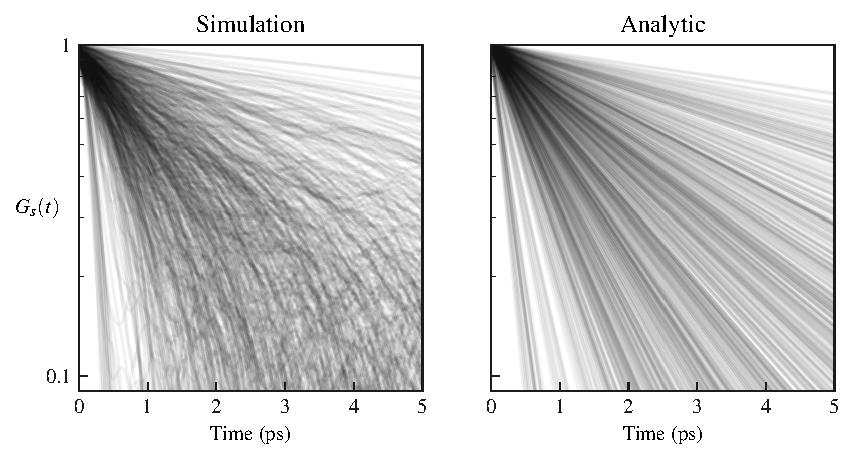
\includegraphics[width=\textwidth]{./data/plots/lifetimes/greenkubo_summary_interpolation_lifetimes.pdf}
	\caption{Fit of mode lifetimes for MgO at 300\,K.}
\end{figure}
